%%%%%%%%%%%%%%%%%%%%%%%%%%%%%%%%%%%%%%%%%
% BEMOSS Landscape Poster
% LaTeX Template
% Version 1.0 (29/03/13)
%
% Created by: Reece 
% Computational Physics and Biophysics Group, Jacobs University
% https://teamwork.jacobs-university.de:8443/confluence/display/CoPandBiG/LaTeX+Poster
% 
% Further modified by:
% Nathaniel Johnston (nathaniel@njohnston.ca)
%
% This template has been downloaded from:
% http://www.LaTeXTemplates.com
%
% License:
% CC BY-NC-SA 3.0 (http://creativecommons.org/licenses/by-nc-sa/3.0/)
%
%%%%%%%%%%%%%%%%%%%%%%%%%%%%%%%%%%%%%%%%%

%----------------------------------------------------------------------------------------
%	PACKAGES AND OTHER DOCUMENT CONFIGURATIONS
%----------------------------------------------------------------------------------------

\documentclass[final]{beamer}

\usepackage[scale=1.24]{beamerposter} % Use the beamerposter package for laying out the poster

\usepackage{tikz}
\usepackage{todonotes}
\usepackage{epstopdf}
\epstopdfsetup{suffix = {}}
\usepackage{hyperref}
\usepackage{subfigure}  % Written by Steven Douglas Cochran
\usepackage{amssymb,amsmath,bm}    % From the American Mathematical Society
\usepackage{siunitx} % for units like degree, ...
\sisetup{unitsep=\cdot,binary-units=true}
\usepackage{mathtools}
\usepackage{xcolor,soul}
\usepackage{geometry}
\usetheme{confposter} % Use the confposter theme supplied with this template

\setbeamercolor{block title}{fg=BUred,bg=white} % Colors of the block titles
\setbeamercolor{block body}{fg=black,bg=white} % Colors of the body of blocks
\setbeamercolor{block alerted title}{fg=BUred,bg=gray!70} % Colors of the highlighted block titles
\setbeamercolor{block alerted body}{fg=black,bg=gray!10} % Colors of the body of highlighted blocks


% Many more colors are available for use in beamerthemeconfposter.sty

%-----------------------------------------------------------
% Define the column widths and overall poster size
% To set effective sepwid, onecolwid and twocolwid values, first choose how many columns you want and how much separation you want between columns
% In this template, the separation width chosen is 0.024 of the paper width and a 4-column layout
% onecolwid should therefore be (1-(# of columns+1)*sepwid)/# of columns e.g. (1-(4+1)*0.024)/4 = 0.22
% Set twocolwid to be (2*onecolwid)+sepwid = 0.464
% Set threecolwid to be (3*onecolwid)+2*sepwid = 0.708

\newlength{\sepwid}
\newlength{\onecolwid}
\newlength{\twocolwid}
\newlength{\threecolwid}
\setlength{\paperwidth}{48in} % A0 width: 46.8in
\setlength{\paperheight}{36in} % A0 height: 33.1in
\setlength{\sepwid}{0.022\paperwidth} % Separation width (white space) between columns
\setlength{\onecolwid}{0.22\paperwidth} % Width of one column
\setlength{\twocolwid}{0.464\paperwidth} % Width of two columns
\setlength{\threecolwid}{0.708\paperwidth} % Width of three columns
\setlength{\topmargin}{-0.25in} % Reduce the top margin size
\setlength{\leftmargin}{-0.25in}
\setlength{\rightmargin}{-0.25in}

%-----------------------------------------------------------

\usepackage{graphicx}  % Required for including images

\usepackage{booktabs} % Top and bottom rules for tables
%\usepackage{subfigure}

%-----------------------------------------------------------
% TITLE SECTION
%-----------------------------------------------------------

\title{BEMOSS: Building Energy Management Open Source Software} % Poster title

\author{Reece Bachman, Robert O'Malley, Jordan Ingram, Advisor: Dr. Suruz Miah} % Author(s)


\institute{Department of Electrical and Computer Engineering, Bradley University, Peoria IL} %Institution(s)
\vskip -.5cm

%-----------------------------------------------------------
% POSTER CONTENT
%-----------------------------------------------------------

\begin{document}

\addtobeamertemplate{block end}{}{\vspace*{1ex}} % White space under blocks
\addtobeamertemplate{block alerted end}{}{\vspace*{2ex}} % White space under highlighted (alert) blocks

\setlength{\belowcaptionskip}{2ex} % White space under figures
%\setlength\belowdisplayshortskip{2ex} % White space under equations

\begin{frame}[t] % The whole poster is enclosed in one beamer frame

\begin{columns}[t]

\begin{column}{\sepwid}\end{column} % Empty spacer column

\begin{column}{\onecolwid} % The first column

%-----------------------------------------------------------
% OBJECTIVE AND CONTRIBUTION
%-----------------------------------------------------------
\begin{block}{Application}
    \begin{figure}
    \centering
 
    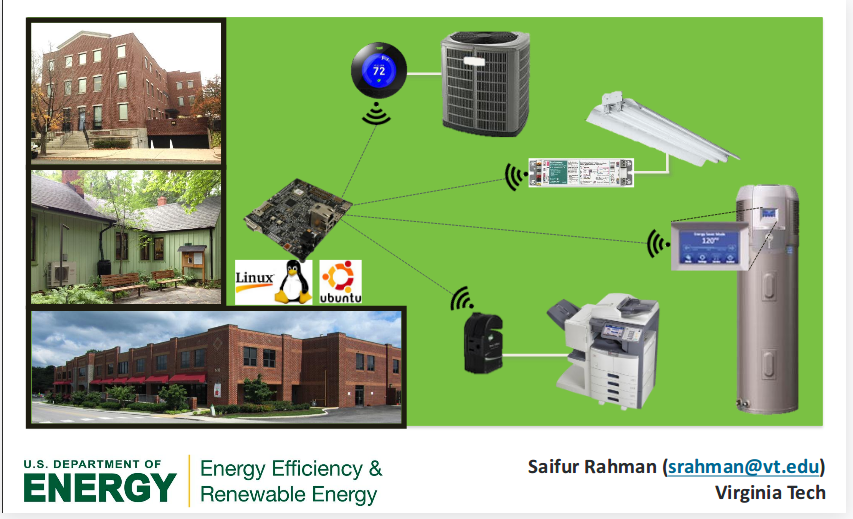
\includegraphics[width=.99\textwidth,keepaspectratio=true]{figs/img/DOE.png}
   \caption{Current BEMOSS Structure}
    \label{fig:MotorCircuit}
    \end{figure}
\end{block}


%-----------------------------------------------------------
% PROBLEM SETUP
%-----------------------------------------------------------
\vskip -1cm
\begin{block}{BEMOSS Overview}
\vskip -1cm
\begin{itemize}
    \item Internet of Things(IoT) control Software
    \item Control entire building worth of devices
    \item Energy friendly environment control 
    \item Developed under the Department of Energy
    \item Supports HVAC, plug loads, fans, and sensors
    \item We are adding the support of a DC motor
\end{itemize}

\begin{figure}
    \centering
    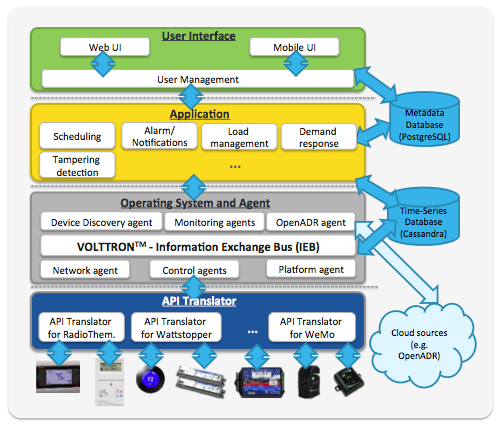
\includegraphics[width=.99\textwidth]{figs/img/BEMOSSv2_SoftwareArchitecture.png}
    \caption{BEMOSS software architecture (courtesy of Department of Energy)}
    \label{fig:my_label}
\end{figure}

\begin{alertblock}{Objectives}
%
\begin{itemize}
    \item Integrate a new device within BEMOSS
    \item Get BEMOSS to run on a embedded computer
    \item Develop and implement an energy saving algorithm to BEMOSS
\end{itemize}
%
\vskip -1cm

\vskip -0.75cm
%\begin{itemize}
 %   \item Create network based motor controller
  %  \item Discover devices on network and talk to relevant ones
   % \item Energy efficient building algorithm research
%\end{itemize}

\end{alertblock}

\vskip -2cm
\end{block}

\end{column} % End of the first column

\begin{column}{\sepwid}\end{column} % Empty spacer column

\begin{column}{\onecolwid} % The second column

%-----------------------------------------------------------
% EKF-SLAM
%-----------------------------------------------------------

\begin{figure}
    \centering
    \fcolorbox{gray!20}{gray!20}{
    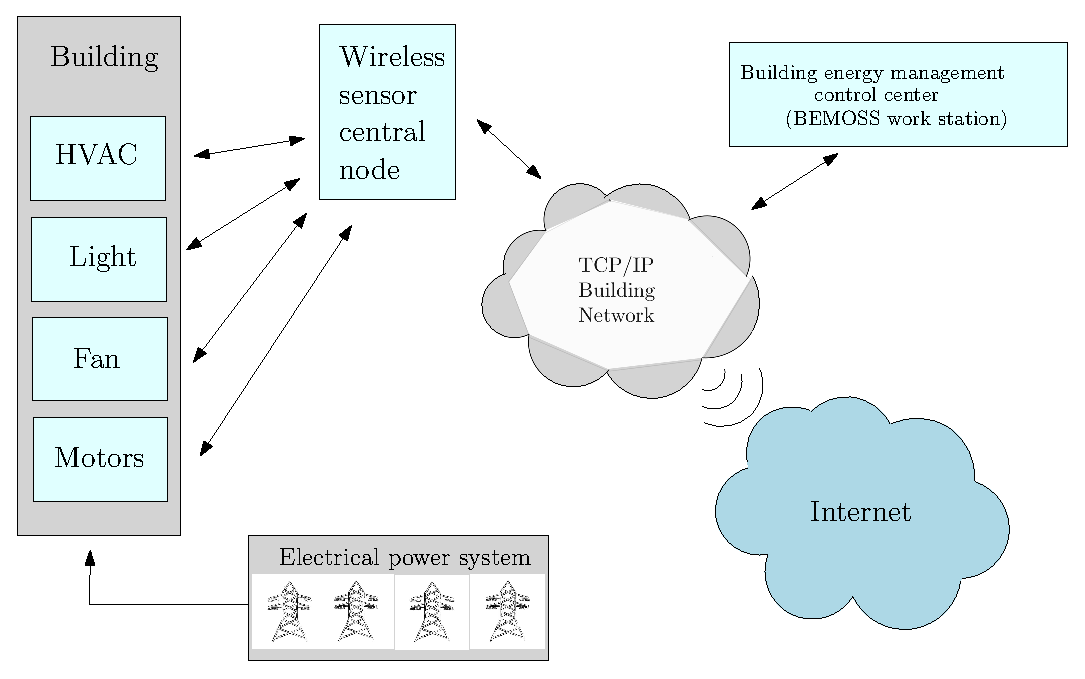
\includegraphics[width=.79\textwidth,keepaspectratio=true]{figs/ipe/HighLevelBemoss.eps}

    }
    \label{fig:MotorCircuit}
    \caption{Proposed BEMOSS structure.}
    \end{figure}
\begin{block}{New IoT Device (Motor) Configuration}
\vskip -0.5cm
\begin{itemize}
 
        \item Central hub to control multiple DC motors 
        \item Facilitates RF communications to DC motors
        \item Controlled via a network 

 \end{itemize}
    %\end{align}
    \begin{figure}
    \centering
    \subfigure[][]{   
    \label{fig:node4-9-Arrows}
    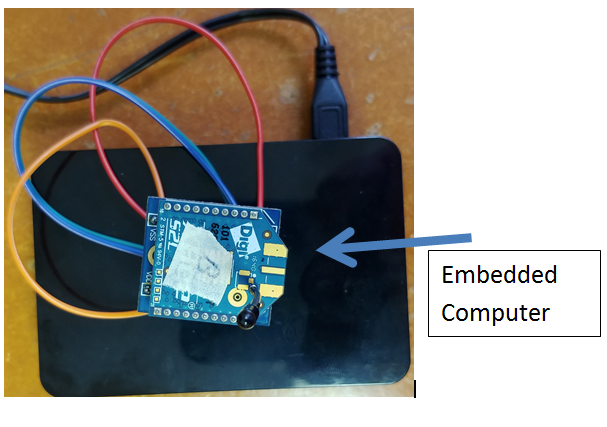
\includegraphics[width=.45\textwidth,keepaspectratio=true]{figs/img/node4-9-Arrows.png}
    }
    \subfigure[][]{
    \label{fig:circuit4-9-Arrows}
        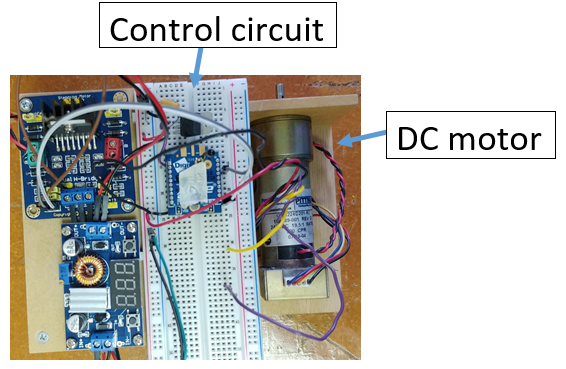
\includegraphics[width=.45\textwidth,keepaspectratio=true]{figs/img/circuit4-9-Arrows.png}
    }
    \label{fig:MotorCircuit}
    \caption{\subref{fig:node4-9-Arrows} IoT central node and~\subref{fig:circuit4-9-Arrows} IoT motor.}
    \end{figure}
  

%\vskip -2.6cm


%\vskip -2.5cm


%-----------------------------------------------------------
% RANGE AND BEARING APPROXIMATION
%-----------------------------------------------------------


\vskip -1cm
\begin{itemize}
    \item Automate curtains and doors
    \item Regulate interior temperatures and privacy 
\end{itemize}
\vskip -.5cm
\begin{figure}
    \centering
    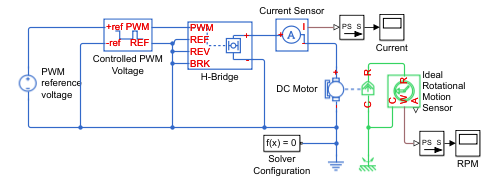
\includegraphics[width=.75\textwidth,keepaspectratio=true]{figs/img/motorModelWithHBridge.png}
    \caption{Simscape Motor Model}
    \label{fig:motorModelWithHBridge}
\end{figure}

\end{block}

\begin{block}{Automatic Detection \& Control}
\vskip -1cm
\begin{itemize}
    \item Discover all devices connected to the network
    \item Deduce which devices we desire to control on the network 
    \item Collect necessary control information 
    \item Connect to desired node
    \item Display control interface 
\end{itemize}

\vskip -.5cm
\begin{figure}
    \centering
    \fcolorbox{gray!20}{gray!20}{
        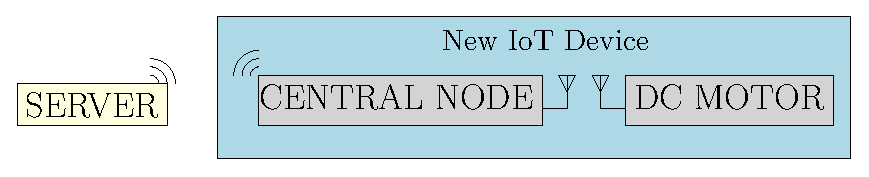
\includegraphics[width=.69\textwidth,keepaspectratio=true]{figs/ipe/Discovery.eps}
    }
    \label{fig:MotorCircuit}
    \caption{Discovery Method}
\end{figure}

\end{block}
\end{column} % End of second column

\begin{column}{\sepwid}\end{column} % Empty spacer column

\begin{column}{\onecolwid} % The third column
%-----------------------------------------------------------
% MOTION CONTROL STRATEGY
%-----------------------------------------------------------

%\vskip -2cm
%-----------------------------------------------------------
% Subsystem Block Diagram
%-----------------------------------------------------------
\begin{block}{Second IoT device (HVAC)}
    \begin{itemize}
        \item Model devices on BEMOSS
        \item Lower energy cost through HVAC control
    \end{itemize}
\end{block}

%-----------------------------------------------------------
% SIMULATION RESULTS
%-----------------------------------------------------------

%\begin{block}{Control Algorithm}
%\vskip -1cm


%Before implementing the algorithm, it was simulated using the industry standard robot simulator V-REP. With numerous robot models available, V-REP is able to accurately and consistently produce like those expected in real--world scenarios. Preliminary simulation results can be seen in Fig.~\ref{fig:vrepResults}.

\begin{figure}
    \subfigure[][]{
    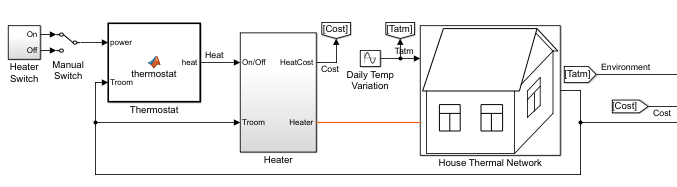
\includegraphics[width=.95\textwidth,keepaspectratio=true]{figs/img/houseModel.PNG}
    \label{fig:houseModel}
    }
    %\subfigure[][]{
    %\includegraphics[width=.46\textwidth,keepaspectratio=true]{figs/matlab/sim1/finalTrajectory_sim1}
    %\label{fig:vrepdata1}
    %}
    \subfigure[][]{
          %\missingfigure{Insert figure.}
     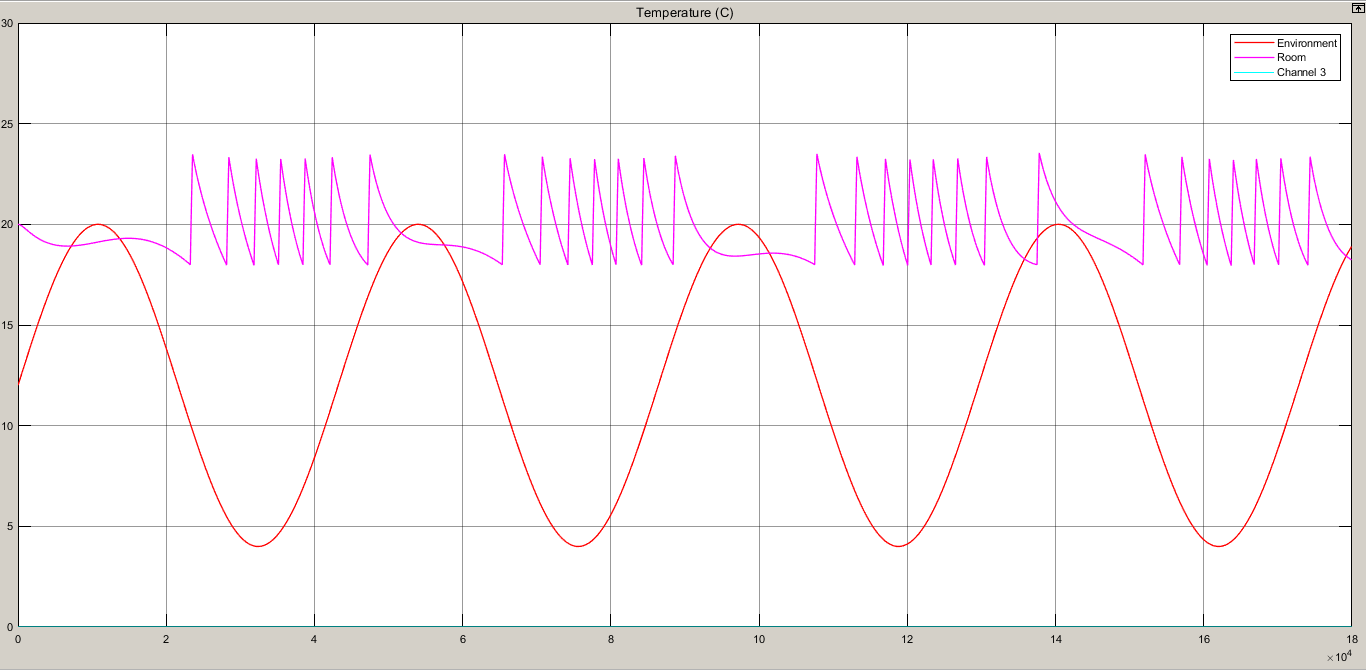
\includegraphics[width=.99\textwidth,keepaspectratio=true]{figs/img/houseModelData.PNG}
    \label{fig:houseData}
    }
    \caption{\subref{fig:houseModel} Simulink Model of One Room House and~\subref{fig:houseData} Temperature of House}
    \label{fig:vrepResults}
\end{figure} %
\vskip -1cm

%\end{block}
\begin{figure}
    \centering
        %\missingfigure{Insert figure.}
     \boxed{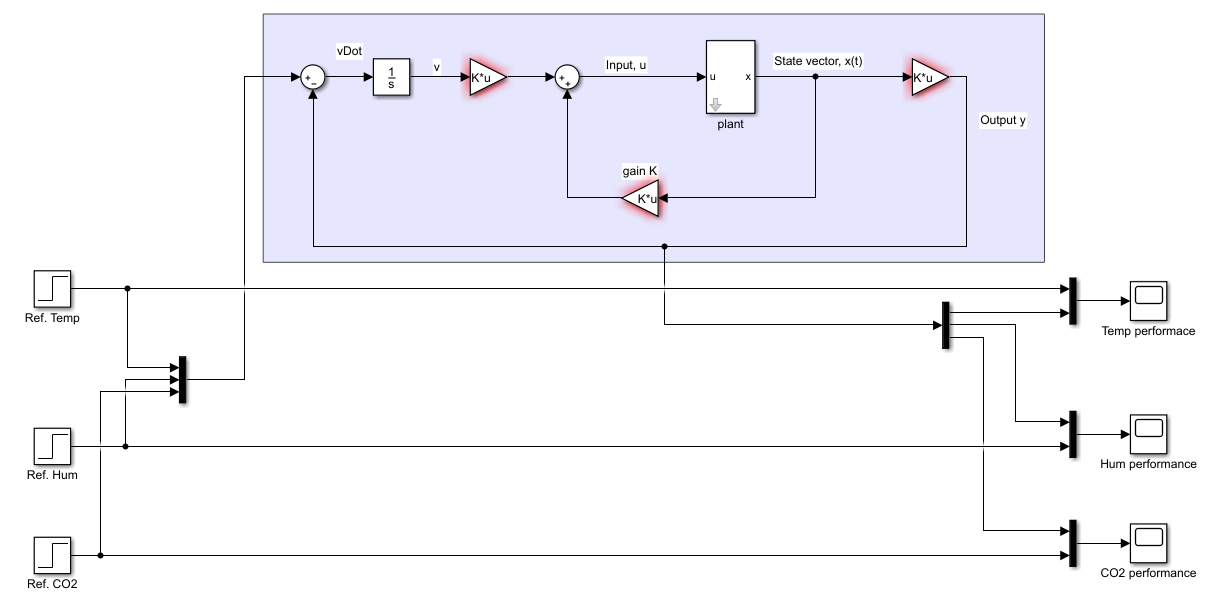
\includegraphics[width=.92\textwidth,keepaspectratio=true]{figs/img/LQRHVAC.PNG}}
    \label{fig:subsystem}
    \caption{Block Diagram for HVAC Control}
\end{figure}

\begin{equation}
    u(t) = -Kx(t) + K_lv(t)
\end{equation}
\begin{equation}
    \Dot{v}(t) = r - Cx(t)
\end{equation}
\begin{itemize}
    \item Controls temperature, humidity, and $CO_2$
    \item Models a one room system
    \item Linear Quadratic Regulator(LQR) control design
\end{itemize}

\end{column} % End of third column

\begin{column}{\sepwid}\end{column}

\begin{column}{\onecolwid} % The fourth column

%-----------------------------------------------------------
% EXPERIMENTAL RESULTS
%-----------------------------------------------------------


\begin{block}{Experimental Results}
\vskip -1cm
\begin{itemize}
    \item Controlled wireless motor over the internet
    \item Controlled WeMo plug through BEMOSS server 
    \item Developed energy saving algorithm 
\end{itemize}
\vskip -.5cm
%The system's performance was tested by having the Pioneer 3-DX navigate through a set of waypoints on the ground while estimating its own pose as well as the positions of beacons distributed throughout the environment. The system can be accessed through ROS, promoting modularity since are no dependencies between modules for communication. Essentially, the robot's pose, the position of the XBee radios, and error information can be monitored in real-time from a remote location. 


\begin{figure}
    \centering
    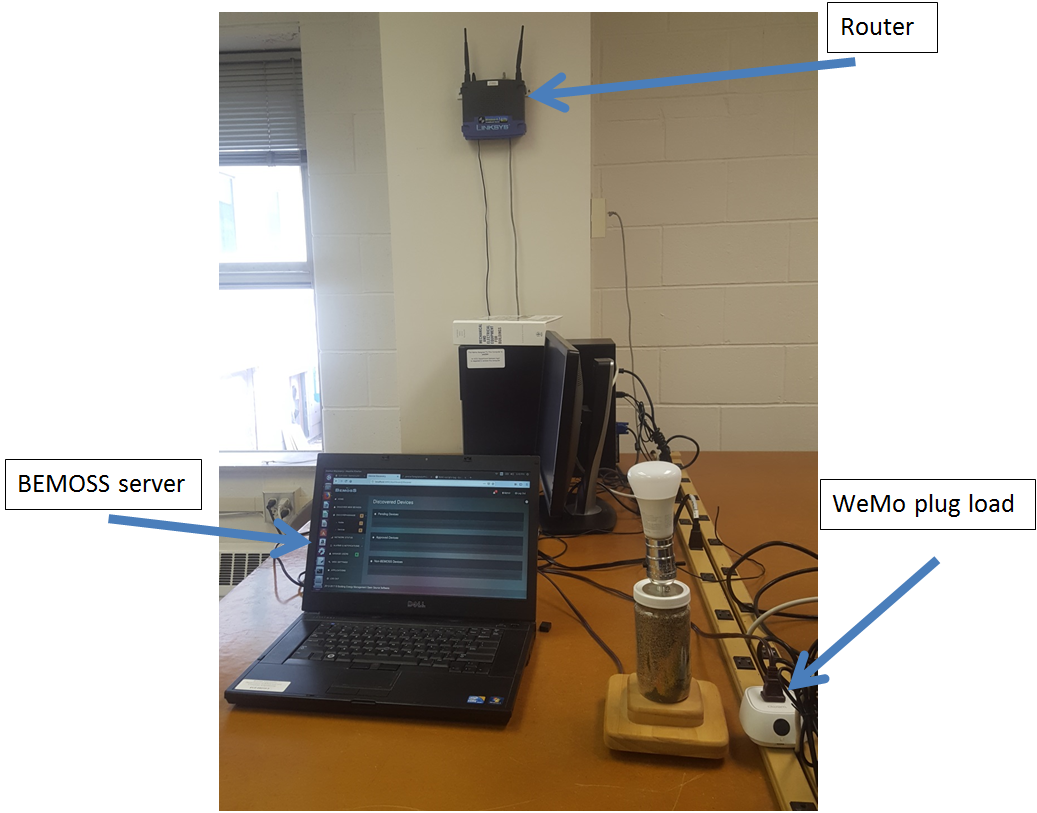
\includegraphics[width=.75\textwidth,keepaspectratio=true]{figs/img/Setup.png}
    \label{fig:my_label}
        \caption{BEMOSS System}
\end{figure}

\begin{figure}
    \centering
    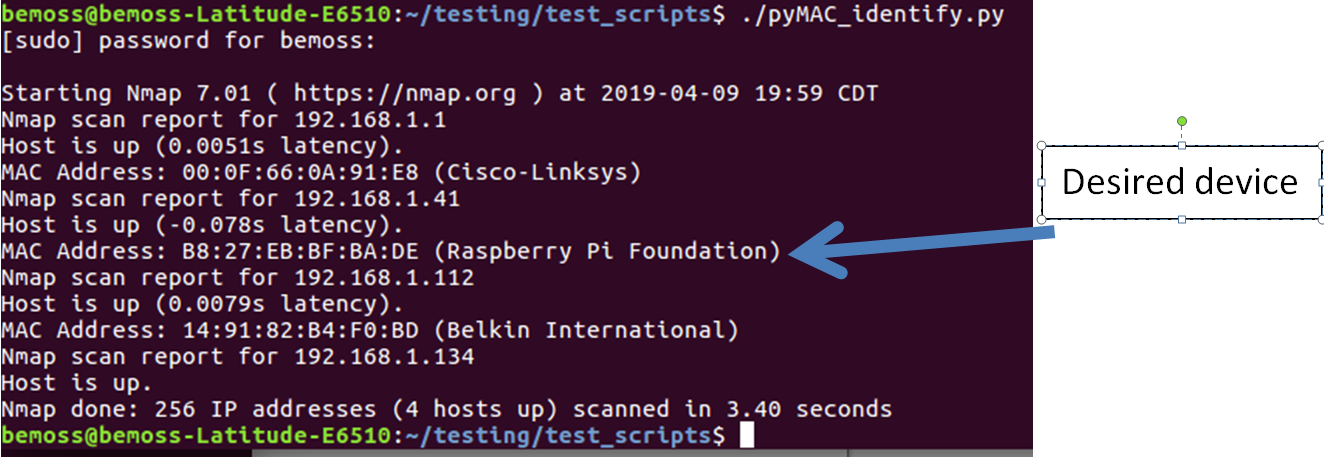
\includegraphics[width=.75\textwidth,keepaspectratio=true]{figs/img/Identify.png}
    \caption{Discovered Devices on Network}
    \label{fig:my_label}
\end{figure}
\begin{figure}
    \centering
    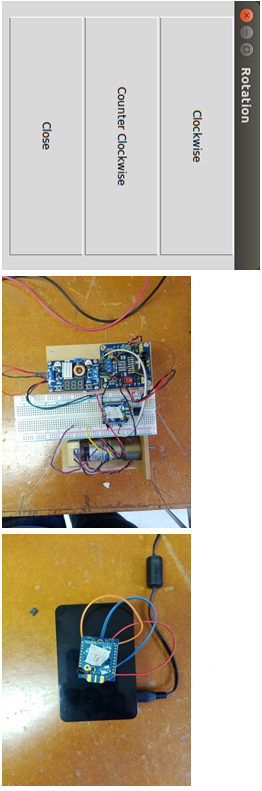
\includegraphics[width=.25\textwidth,keepaspectratio=true, angle=-270]{figs/img/three.png}
    \label{fig:my_label}
        \caption{IoT Motor GUI}
\end{figure}

\begin{figure}
    \centering
    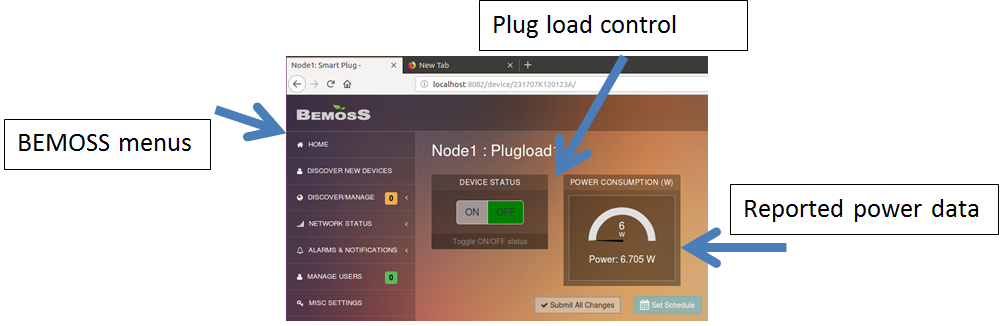
\includegraphics[width=.99\textwidth,keepaspectratio=true]{figs/img/PlugloadData-Arrows.png}
    \caption{Data from Plug load}
   \label{fig:MotorCircuit}

\end{figure}





%Similar to the result seen in simulation, the beacon position estimation error decreases overall as iterations increase. The periodic increases in error result from the position of the mobile robot within the environment and the influence of the environment on measurement accuracy.

\end{block}

%\begin{block}{Conclusion}

%As seen in the experimental results, this system brings moderate accuracy considering its implementation. With a total cost of around \$140 for the system mounted on the mobile robot and around \$23 for the beacons, this system is much more attainable for those conducting research in mapping and localization algorithms and inexpensive to scale to commercial applications.

%\end{block}

%-----------------------------------------------------------
% Conclusion and Future Work
%-----------------------------------------------------------

\begin{alertblock}{Summary and Future Work}
\begin{itemize}
    \item Interface a motor positional feedback system
    \item Integrate current energy saving algorithm with curtain toggle abilities
    \item Test the efficiency of our newly developed system 
\end{itemize}


\end{alertblock}

\end{column} % End of the fourth column

\end{columns} % End of all the columns in the poster

\end{frame} % End of the enclosing frame

\end{document}

%%% Local Variables:
%%% mode: latex
%%% TeX-master: t
%%% End:
